\documentclass[12pt]{article}

\usepackage{amsmath}
\usepackage{hyperref}
\usepackage{graphicx}
\usepackage{float}
\usepackage{caption}
\usepackage{listings}
\usepackage{xcolor}

% Define colors
\colorlet{punct}{red!60!black}
\definecolor{background}{RGB}{240, 248, 255} % Pale Blue
\definecolor{delim}{RGB}{20,105,176}
\colorlet{numb}{magenta!60!black}

% Define JSON language
\lstdefinelanguage{json}{
    basicstyle=\normalfont\ttfamily,
    numbers=left,
    numberstyle=\scriptsize,
    stepnumber=1,
    numbersep=8pt,
    showstringspaces=false,
    breaklines=true,
    frame=lines,
    backgroundcolor=\color{background},
    literate=
     *{0}{{{\color{numb}0}}}{1}
      {1}{{{\color{numb}1}}}{1}
      {2}{{{\color{numb}2}}}{1}
      {3}{{{\color{numb}3}}}{1}
      {4}{{{\color{numb}4}}}{1}
      {5}{{{\color{numb}5}}}{1}
      {6}{{{\color{numb}6}}}{1}
      {7}{{{\color{numb}7}}}{1}
      {8}{{{\color{numb}8}}}{1}
      {9}{{{\color{numb}9}}}{1}
      {:}{{{\color{punct}{:}}}}{1}
      {,}{{{\color{punct}{,}}}}{1}
      {\{}{{{\color{delim}{\{}}}}{1}
      {\}}{{{\color{delim}{\}}}}}{1}
      {[}{{{\color{delim}{[}}}}{1}
      {]}{{{\color{delim}{]}}}}{1},
}

\setlength{\parskip}{1em}

\lstset{frame=single, showstringspaces=false, columns=fixed, basicstyle={\ttfamily}, commentstyle={\it}, numbers=left, tabsize=4}

\definecolor{codebackground}{RGB}{240, 248, 255} % Pale Blue
\definecolor{codecomment}{RGB}{106,153,85}
\definecolor{codekeyword}{RGB}{30,30,255}
\definecolor{codestring}{RGB}{163,21,21}
\definecolor{codenumber}{RGB}{100,100,100}

\lstdefinestyle{modernstyle}{
    backgroundcolor=\color{codebackground},
    commentstyle=\color{codecomment},
    keywordstyle=\color{codekeyword},
    numberstyle=\tiny\color{codenumber},
    stringstyle=\color{codestring},
    basicstyle=\ttfamily\footnotesize\color{black},
    breakatwhitespace=false,
    breaklines=true,
    captionpos=b,
    keepspaces=true,
    numbers=left,
    numbersep=5pt,
    showspaces=false,
    showstringspaces=false,
    showtabs=false,
    tabsize=4
}

\lstset{style=modernstyle}

\begin{document}

\begin{titlepage}
\centering

\includegraphics[width=0.5\textwidth]{images/logo_ufr.png}\par\vspace{1cm}
\vspace{1.5cm}
{\huge\bfseries ExaMA WP1 - Vegetation\par}
\vspace{2cm}
{\Large Giulio Carpi Lapi, Pierre-Antoine Senger\par}
\vfill
supervised by\par
Pierre Alliez and Vincent Chabannes

\vfill

% Bottom of the page
{\large Date: \today\par}
\end{titlepage}

\tableofcontents
\newpage

\section{Introduction}
Urban areas are complex ecosystems influenced by various factors, among which 
vegetation, especially trees, holds significant importance. Trees play a crucial 
role in shaping microclimates, reducing energy consumption, and enhancing overall 
livability\cite{TIR4sTREEt}. This project aims to integrate vegetation, specifically trees, into 3D 
geometric models of urban environments to improve the accuracy and realism of thermal 
and energy simulations. Utilizing data from open sources like \texttt{OpenStreetMap},
we identified tree positions and attributes and developed a library of 3D tree
models for integration into terrain meshes.

The project follows a roadmap with defined milestones to deliver versions
\texttt{V0}, \texttt{V1}, and \texttt{V2} by specified  deadlines.

\subsection{Main Objectives}

The primary objective is to enhance the accuracy of thermal and energy
simulations of a given area.

Specific objectives include:
\begin{itemize}
    \item Extracting tree data from \texttt{OpenStreetMap}
    \item Generating 3D tree models.
    \item Integrating tree models into terrain meshes.
    \item Simulating how trees influence energy consumption and microclimates.
    \item Optimizing computational efficiency
    \item Delivering versions \texttt{V0}, \texttt{V1}, and \texttt{V2} by specified deadlines
\end{itemize}

\begin{figure}[H]
    \centering
    \begin{minipage}{0.45\textwidth}
        \centering
        \includegraphics[width=\textwidth]{images/TreeShade.png}
        \captionsetup{font={scriptsize}}
        \caption{Tree providing shade to a building \cite{img:TreeShade}.}
    \end{minipage}\hfill
    \begin{minipage}{0.45\textwidth}
        \centering
        \includegraphics[width=\textwidth]{images/heat_street.png}
        \captionsetup{font={scriptsize}}
        \caption{Thermal image of a street depicting heat distribution \cite{img:street_thermography}.}
    \end{minipage}
\end{figure}

Computational modeling has advanced significantly, enabling the simulation of thermal 
and energy performance in urban environments. However, integrating vegetation into 
these models presents challenges due to the complexity of obtaining accurate tree data 
and representing their geometry efficiently\cite{AdTree}.

\newpage

\subsection{Challenges}
This project aims to address these challenges by developing a methodology for 
integrating trees into 3D urban models. Leveraging data from \texttt{OpenStreetMap},
the  project will identify tree positions and attributes, generate a library of 3D tree 
models, and integrate them into terrain meshes for comprehensive simulations while
ensuring computational efficiency.

\subsection{Data Formats and Structure}
Tree data will be sourced from \texttt{OpenStreetMap} and processed into formats suitable for 
integration into our models, such as \texttt{.stl}, \texttt{.csv}, and \texttt{.json}.
We aim to ensure watertight triangulation consistent with the Finite Element Method
(FEM) for accurate simulations.  

The \texttt{stl} format\cite{stl_format} is a widely used format for 3D printing and computer-aided design (CAD)
software. It represents 3D models as a collection of triangular facets, making it
suitable for our geometric modeling purposes.
The \texttt{ASCII} versions is defined as :
\begin{lstlisting}
solid name
facet normal ni nj nk
    outer loop
        vertex v1x v1y v1z
        vertex v2x v2y v2z
        vertex v3x v3y v3z
    endloop
endfacet
....
endsolid name
\end{lstlisting}
But for efficiency we will use the \texttt{stl} format in its \textbf{binary form}.
\subsection{Software and Libraries}
To source our data, we'll utilize the \texttt{Overpass API} \cite{overpass} alongside
\texttt{curl} \cite{curl} to access and leverage information from \texttt{OpenStreetMap}.
For geometric modeling, we will utilize the \texttt{CGAL} library, known for its efficiency and 
reliability in geometric computation\cite{cgal}. Shading calculations will be performed using the 
\texttt{Feel++} \cite{feel++} library, which specializes in solving Partial Differential Equations (PDEs) 
essential for simulating light and shade on 3D objects.

\subsection{GitHub Repository}
We created a \href{https://github.com/master-csmi/2024-m1-vegetation}{GitHub} repository to manage the project and facilitate collaboration.
The repository contains the project's code, documentation, and resources. It will be
updated regularly to reflect the progress and changes made during the project's
development.

\subsection{Roadmap}
The roadmap we defined includes the following milestones and issues:

\begin{figure}[H]
    \centering
    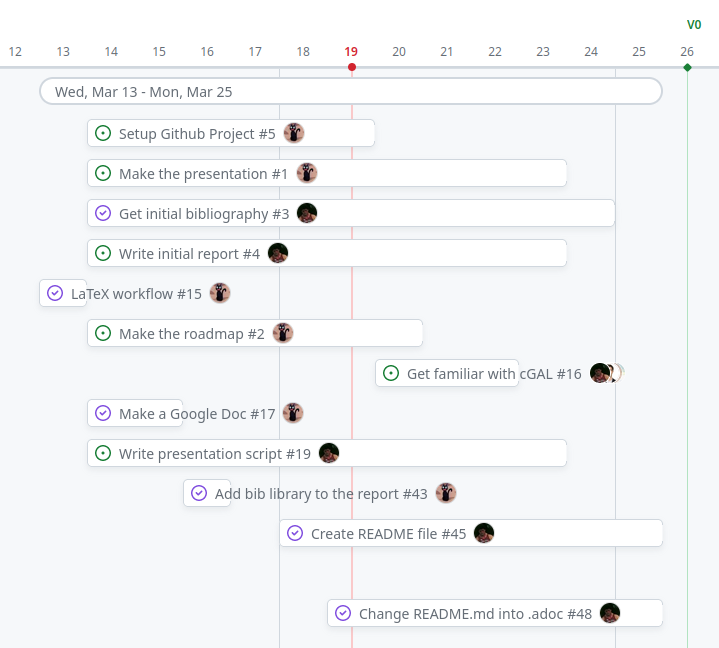
\includegraphics[width=1\textwidth]{images/roadmap_v0.png}
    \captionsetup{font={scriptsize}}
    \caption{Roadmap for V0}
\end{figure}

\begin{figure}[H]
    \centering
    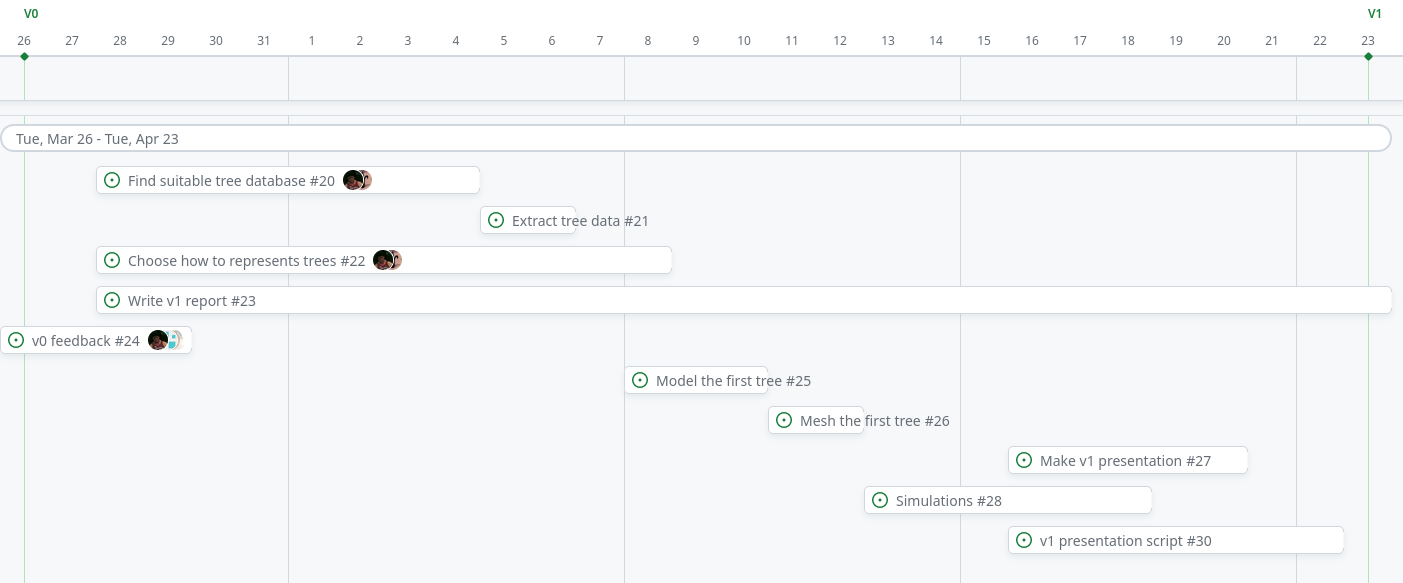
\includegraphics[width=1\textwidth]{images/roadmap_v1.png}
    \captionsetup{font={scriptsize}}
    \caption{Roadmap for V1}
\end{figure}

\begin{figure}[H]
    \centering
    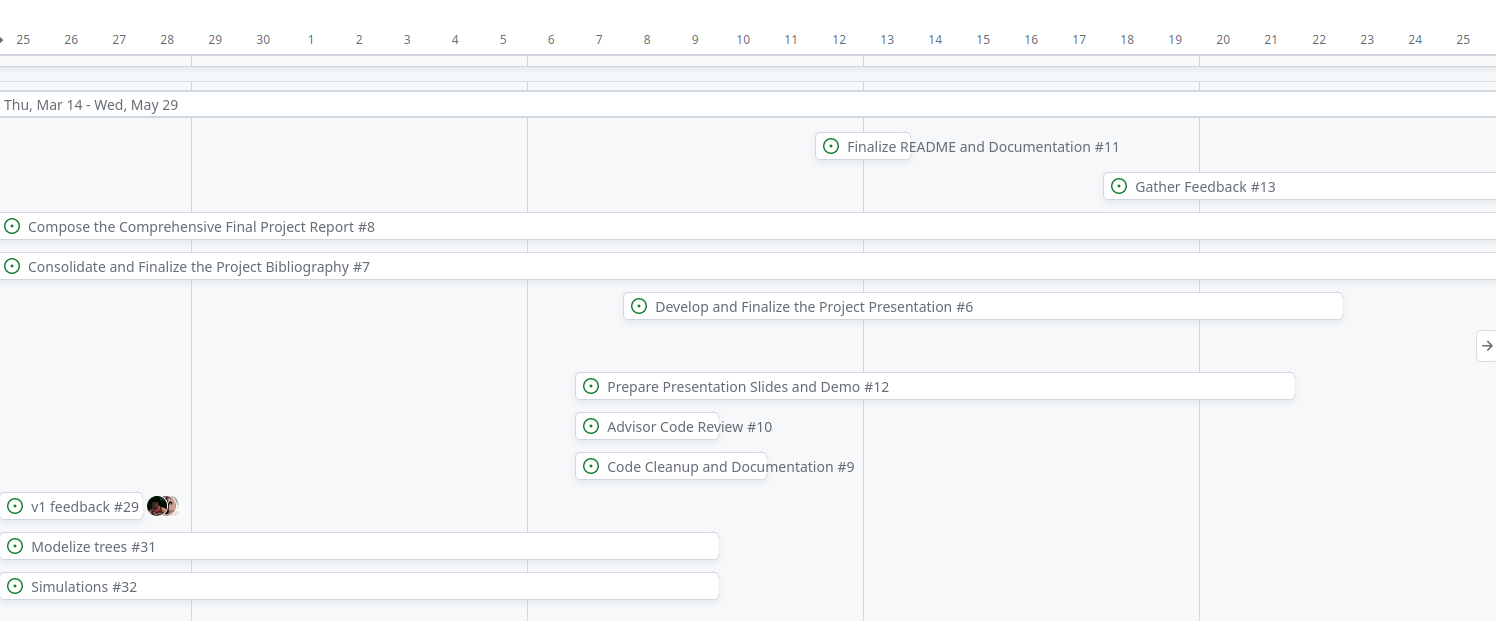
\includegraphics[width=1\textwidth]{images/roadmap_v2.png}
    \captionsetup{font={scriptsize}}
    \caption{Roadmap for V2}
\end{figure}

\newpage

\section{Methodology}

\subsection{Data Acquisition}
A \textit{config.json} file will be available for the user to specify the area of
interest. The file contains the latitude and longitude of two points, A and B,
which define a bounding box.

Here's an example of the \textit{config.json} file for the Strasbourg, France
city center:

\begin{lstlisting}[language=json]
{
  "A": {
    "latitude": 48.58868,
    "longitude": 7.75168
  },
  "B": {
    "latitude": 48.58548,
    "longitude": 7.75455
  },
  "new_query": true,
  "LOD": 0,
  "KNN_dist": 50,
  "output_name": "republique"
}
\end{lstlisting}

Where :
\begin{itemize}
    \item \texttt{A(lat, lon)} represent the top left corner of the box representing the area in OpenStreetMap.
    \item \texttt{B(lat, lon)} represent its bottom right corner.
    \item \texttt{new\_query} is a boolean instruction if data need to be retrieved again or using current one (if it exists).
    \item \texttt{LOD} is the level of details of the meshes (0, 1, 2 or 3)
    \item \texttt{KNN\_dist} is the distance in meter to use to compute the height of the tree when it's missing.
    \item \texttt{output\_name} is the name of the output file representing the unions of the tree meshes.
\end{itemize}

This configuration file will be updated along the way to include more options
as needed such as mesh level of detail (LOD), seasons for the density of leaves,
etc.

We will then use the \texttt{Overpass API} to query \texttt{OpenStreetMap}
for all the available tree data within the specified bounding box.
The data will be stored in a \textit{.json} file.

\newpage
Here's an example of the result of the query for one tree:

\begin{lstlisting}[language=json]
{
    "type": "node",
    "id": 10161978695,
    "lat": 48.5872478,
    "lon": 7.7548520,
    "tags": {
        "circumference": "78.54",
        "diameter_crown": "5",
        "genus": "Tilia",
        "height": "10",
        "natural": "tree",
        "ref": "27466",
        "source": "data.strasbourg.eu - patrimoine_arbore",
        "source:date": "2022-01-02",
        "species": "Tilia euchlora x"
    }
}
\end{lstlisting}

We will especially use the \texttt{position} of the tree (latitude and longitude),
its \texttt{height}, the \texttt{diameter of its foliage}, and the \texttt{species}
to generate the 3D tree models.

\subsection{Tree Library}

\subsection{Tree Model Generation}
Using CGAL Alpha Wrapper \cite{cgal_alpha_wrapper}, 3D tree models will be generated based on the extracted data. Various 
Levels of Detail (LOD) will be considered to balance model complexity and computational 
efficiency depending on the application.

Each tree model will have a CGAL \href{https://doc.cgal.org/latest/Surface_mesh/classCGAL_1_1Surface__mesh.html}{Mesh} 
wrapper object that will contain the tree's
mesh and its position in the 3D space. To ensure efficient computation, this 
mesh object will be created using a predefined LOD tree reference model, it will
be scaled and translated to match the tree's real life height and position.

\begin{figure}[H]
    \centering
    \begin{minipage}{0.45\textwidth}
        \centering
        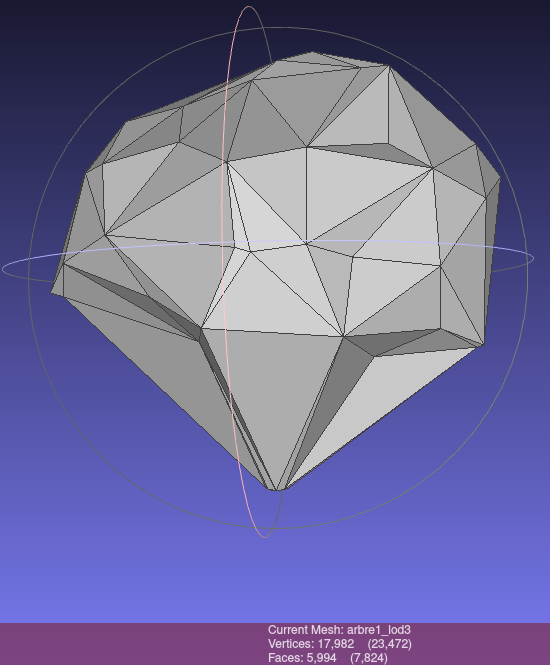
\includegraphics[width=\textwidth]{images/lod0.png}
        \captionsetup{font={scriptsize}}
        \caption{A reference mesh tree for LOD 0.}
    \end{minipage}\hfill
    \begin{minipage}{0.45\textwidth}
        \centering
        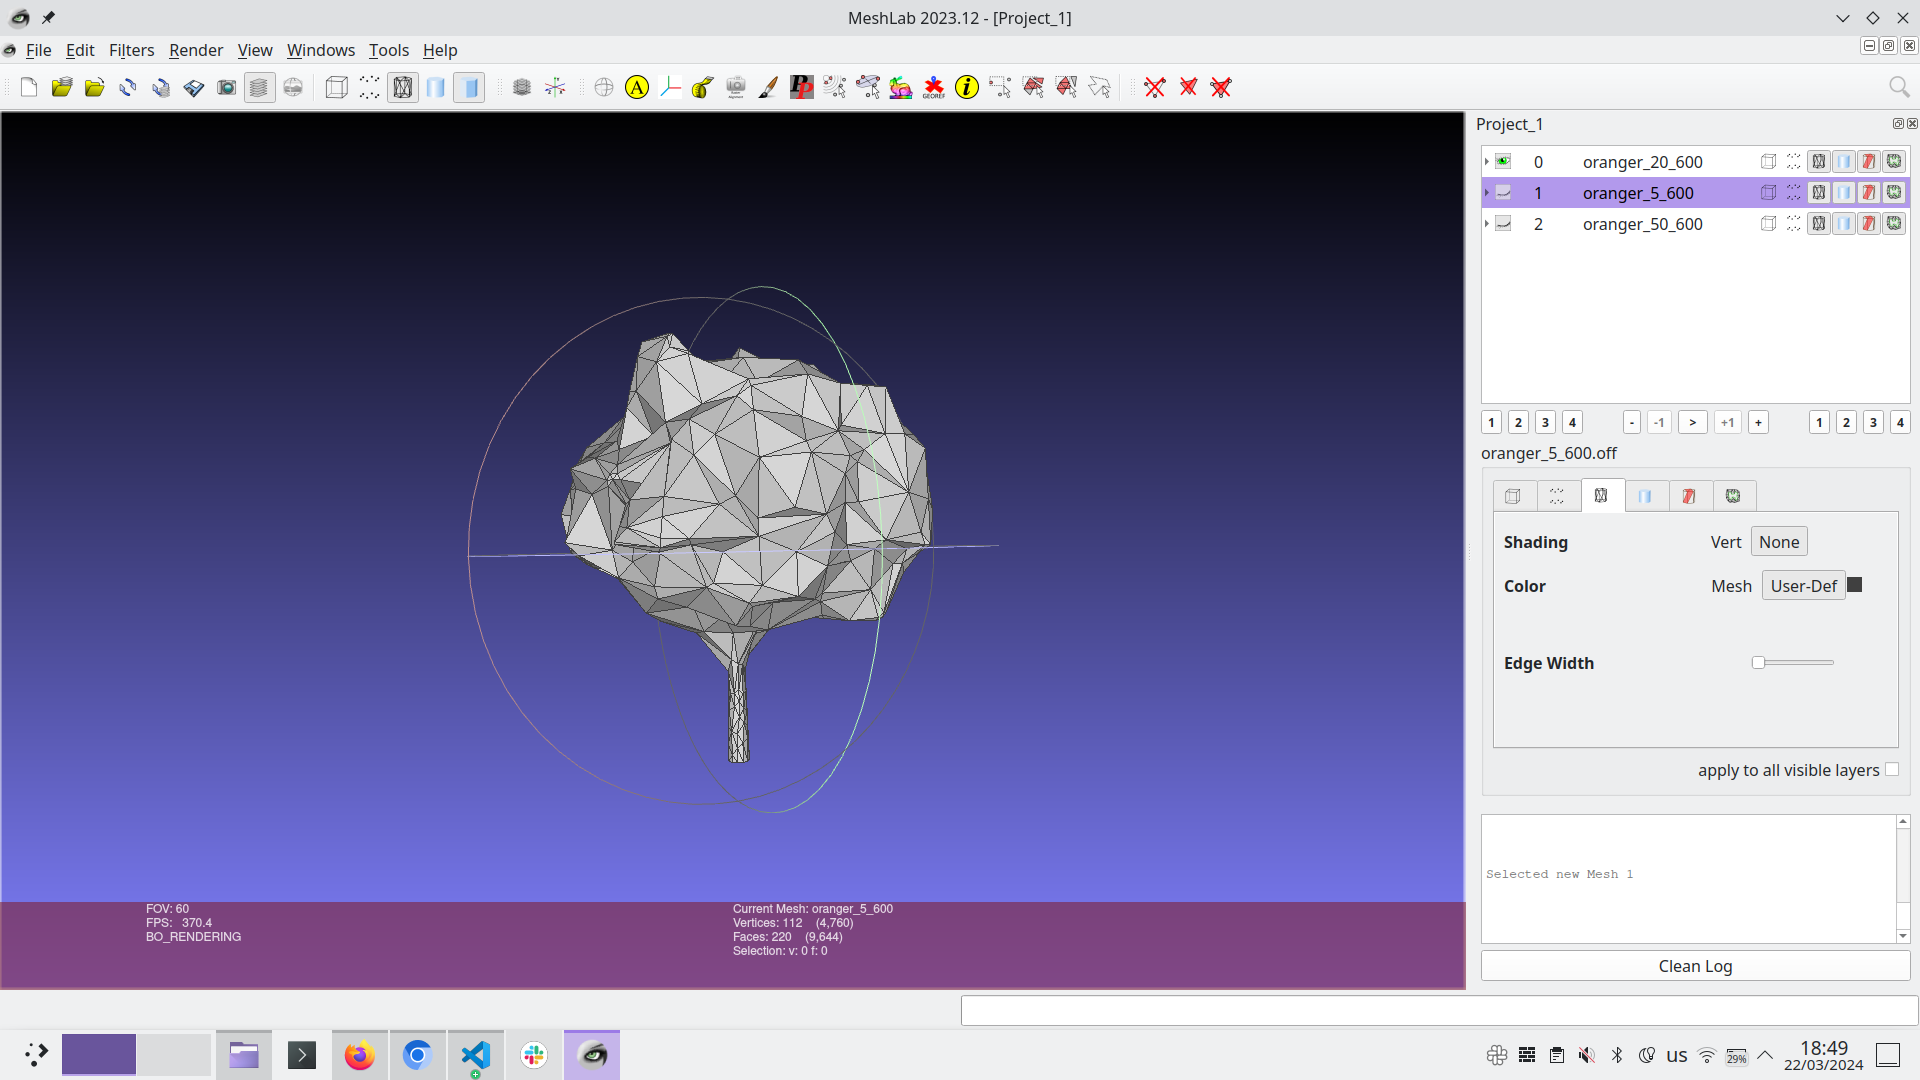
\includegraphics[width=\textwidth]{images/lod1.png}
        \captionsetup{font={scriptsize}}
        \caption{A reference mesh tree for LOD 1.}
    \end{minipage}
\end{figure}

\begin{figure}[H]
    \centering
    \begin{minipage}{0.45\textwidth}
        \centering
        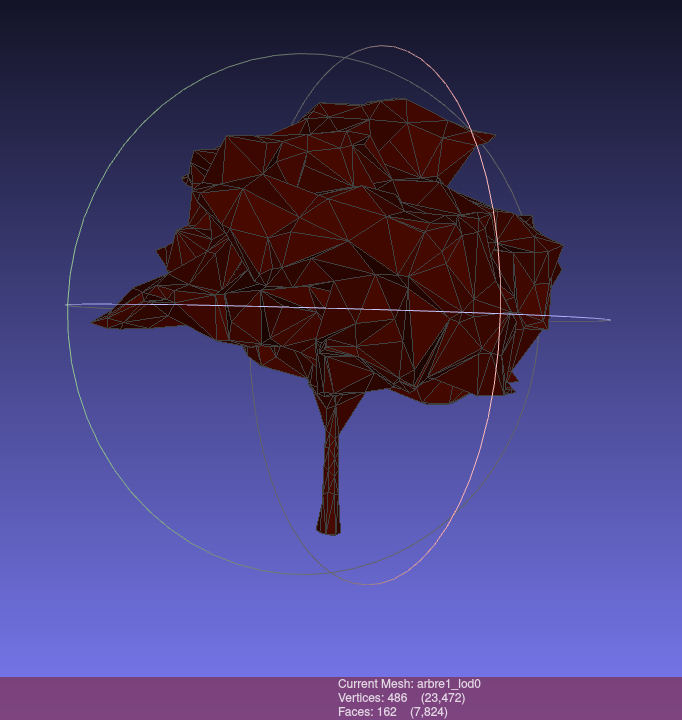
\includegraphics[width=\textwidth]{images/lod2.png}
        \captionsetup{font={scriptsize}}
        \caption{A reference mesh tree for LOD 2.}
    \end{minipage}\hfill
    \begin{minipage}{0.45\textwidth}
        \centering
        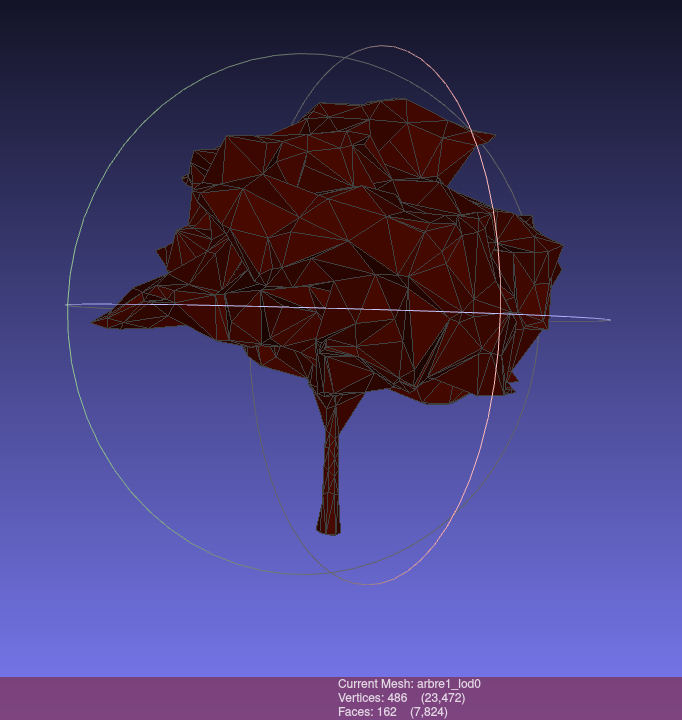
\includegraphics[width=\textwidth]{images/lod3.png}
        \captionsetup{font={scriptsize}}
        \caption{A reference mesh tree for LOD 3.}
    \end{minipage}
\end{figure}

The case where not enough data is available for a tree will need to be handled
as well. For example, we could use a k-nearest neighbors algorithm \cite{k-NN} approach to
decide the tree's metadata (species, height, leave density, etc.) based on the
surrounding trees.

To ensure precise integration into the terrain mesh (especially for large area), the tree models coordinates
(latitude, longitude) will be converted to Cartesian coordinates (x, y) using
a Mercator projection\cite{mercator-proj}. To achieve this we will assume the Earth is a geodesic
defined as WGS84 \cite{wgs84} and use the WGS84toCartesian\cite{wgs84_to_cartesian} open source header-only
  library to convert the coordinates.

The union of all the tree meshed need to be computed to create a single mesh
and avoid collision between the trees.

Here is an example of the tree mesh union of Place de la République in Strasbourg
using generic trees and LOD 3:

\begin{figure}[H]
    \centering
        \centering
        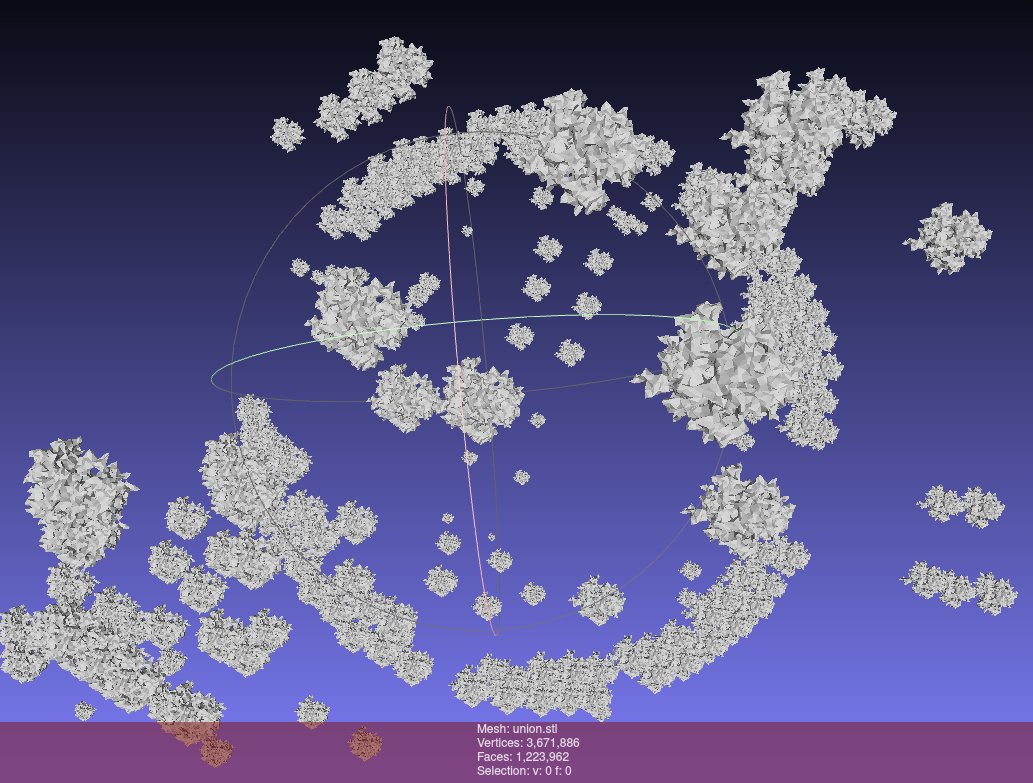
\includegraphics[width=\textwidth]{images/republic_top.png}
        \captionsetup{font={scriptsize}}
        \caption{Top view of Place de la République.}
\end{figure}

\begin{figure}[H]
        \centering
        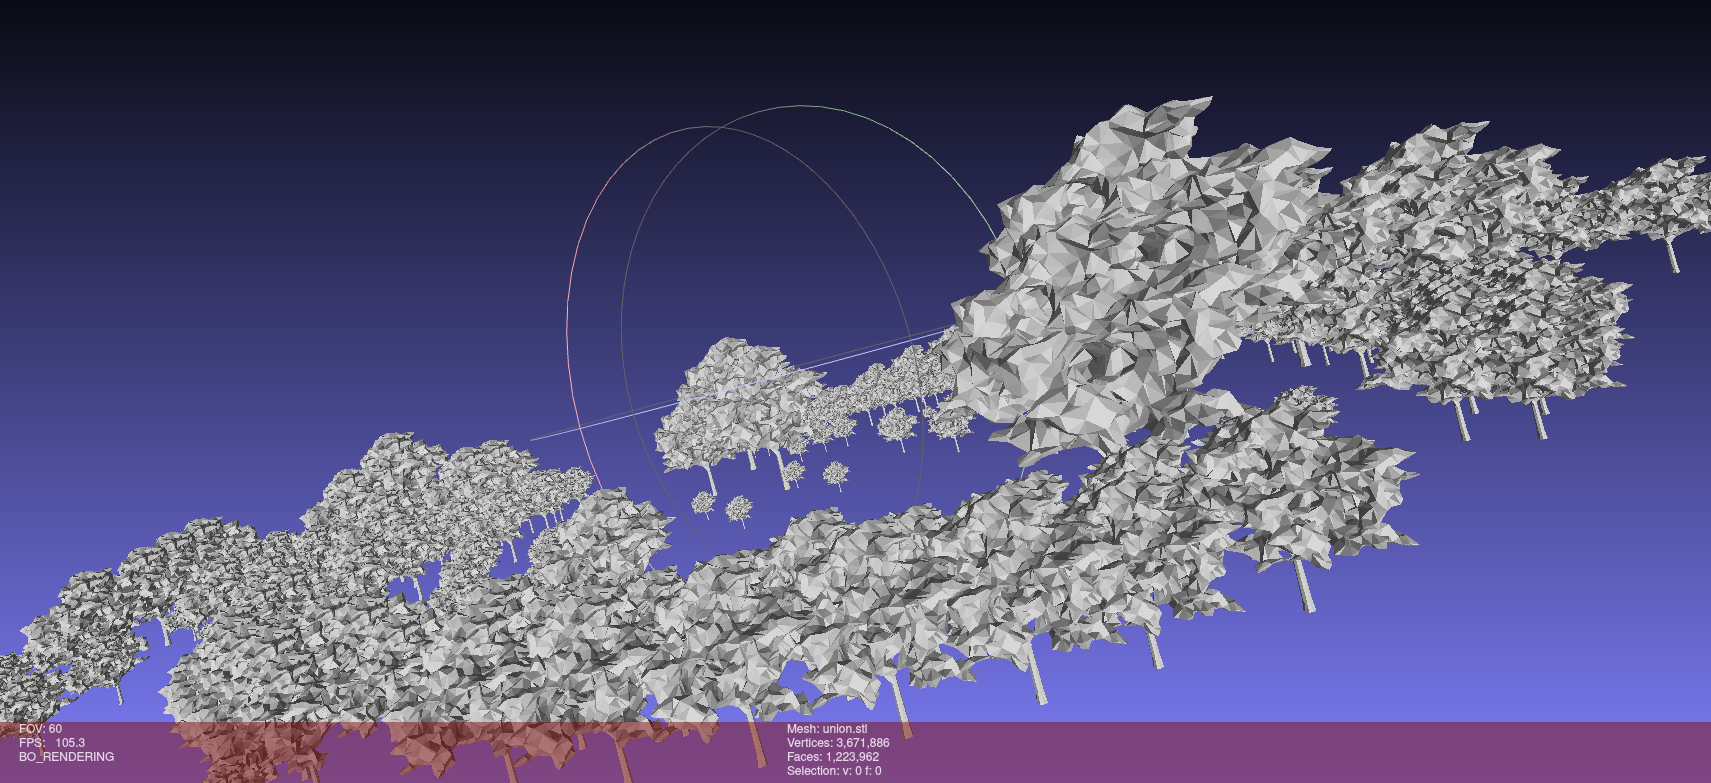
\includegraphics[width=\textwidth]{images/republic.png}
        \captionsetup{font={scriptsize}}
        \caption{Side view of Place de la République.}
\end{figure}

\subsection{Model Integration}
Generated tree models will be integrated into terrain meshes to create comprehensive 
3D urban models. Watertight triangulation consistent with FEM principles will be ensured 
for accurate simulations.

\subsection{Shading Calculations}
Using \texttt{Feel++} ray tracing, shading effects on buildings will be simulated to account for the presence 
of trees and their impact on urban microclimates. Execution time considerations will be 
addressed to optimize computational efficiency.

\section{Implementation}

%  data acquisition
%  tree library
%  tree model generation
%  model integration
%  shading calculations

\section{Results}


\newpage

\section{Conclusion}


\newpage

\section{References}
\bibliographystyle{unsrt}
\bibliography{references}

\end{document}
